\documentclass[10pt]{article}
\usepackage[letterpaper,hmargin=.83in,vmargin=.73in]{geometry}
\usepackage{fontspec,amsmath,booktabs,pgfplots,microtype}
\usepackage[hidelinks,pdftitle={When a partial beach count reverses the direction of change},pdfauthor={ProofRush research team}]{hyperref}
\pgfplotsset{compat=1.18}
\newfontfamily\namefont[Path=../canonne-functional-comparison/fonts/]{ProofRushDirectorJP.otf}
\setlength{\parindent}{0pt}
\setlength{\parskip}{4.6pt}
\newcommand{\para}[1]{\medskip\textbf{#1}\enspace}
\newcommand{\src}[2]{\href{#1}{[#2]}}
\definecolor{deep}{RGB}{14,67,88}
\definecolor{warm}{RGB}{157,66,28}
\begin{document}
\begin{center}
{\LARGE When a partial beach count reverses\\[2pt] the direction of change\par}
\vspace{6pt}
{\large Evidence from daily removals in South Africa and seasonal surveys in Italy}\\[6pt]
ProofRush research team, directed by Yoshiaki Otsuka ({\namefont 大束良明})\\
{\small 27 November 2026, Japan \quad$\cdot$\quad Research note pending external review}
\end{center}

\begin{abstract}
We examined whether counts from one part of a beach track changes in the total number of objects collected across the surveyed beach. In 19 daily removals on two South African beaches, the upper zone accounted for about 64\% of the period total at each site. Yet five of 17 consecutive changes had opposite signs in the upper zone and across both zones. At uMhlanga, any fixed correction factor incurs at least 57.78\% relative error on one observed day. An independent seasonal series from Italy also contained a reversal after omitting the swash zone. For the South African records we replayed a survey design that retains full removal but counts a random subset of the lower-zone bags. Nine of 19 lower-zone counts sufficed for at least 95\% of assignments to place both site-period totals within 20\% of the observed values. All probabilities refer to these fixed historical counts.
\end{abstract}

\para{Survey question.}
Surveys use different cross-shore boundaries. OSPAR describes a section extending from the waterline to the back of the beach. Meakins et al.\ collected upper and lower zones separately in KwaZulu-Natal so that sources with different coverage could be compared. Their paper already shows that the upper zone dominated only early in the uMhlanga series. Buoninsegni et al.\ independently documented seasonal changes across geomorphological zones on the Adriatic. Here we quantify how much a fixed correction can miss, check whether the sign of change survives a restriction in coverage, and evaluate a way to estimate a period total while retaining full-width collection.
\src{https://www.ospar.org/documents?v=44122}{OSPAR, 2025, \S2.4.2}
\src{https://doi.org/10.1016/j.rsma.2022.102421}{Meakins et al., 2022, \S2 and Fig.\ 3}
\src{https://doi.org/10.3390/w17152173}{Buoninsegni et al., 2025, Appendix A}

\para{Daily removals.}
The Cefas/UKZN team removed litter larger than 5\,mm from two 100\,m sections. We required a record of cleaning the preceding day and a survey at the same site on that date. This gives 21--30 September 2019 at Amanzimtoti (10 visits) and 22--30 September at uMhlanga (nine visits). On each visit let $U$ be the item count from the high tide line to the back of the beach, and let $T$ add the items between that line and the water. Counts sum quantified item categories and exclude weights, descriptions and unquantified pellet records. They reproduce the source paper's full-width range of 134--719 objects and its rounded site means of 543 and 340.
\src{https://doi.org/10.14466/CefasDataHub.95}{Cefas Marine Litter Team et al., 2020, version 3}

\begin{center}
\begin{tabular}{lrrrrr}\toprule
Site & Visits & Upper $U$ & Total $T$ & Period $U/T$ & Daily $U/T$ range\\\midrule
Amanzimtoti & 10 & 3,503 & 5,434 & 64.46\% & 41.41--82.68\%\\
uMhlanga & 9 & 1,952 & 3,061 & 63.77\% & 26.15--97.74\%\\\bottomrule
\end{tabular}
\end{center}

\para{Daily direction and magnitude.}
Four of nine adjacent changes at Amanzimtoti and one of eight at uMhlanga changed sign when counts were restricted to the upper zone. On 25--26 September at uMhlanga, $U$ fell from 247 to 223 while $T$ rose from 274 to 468.

\newpage
\begin{center}
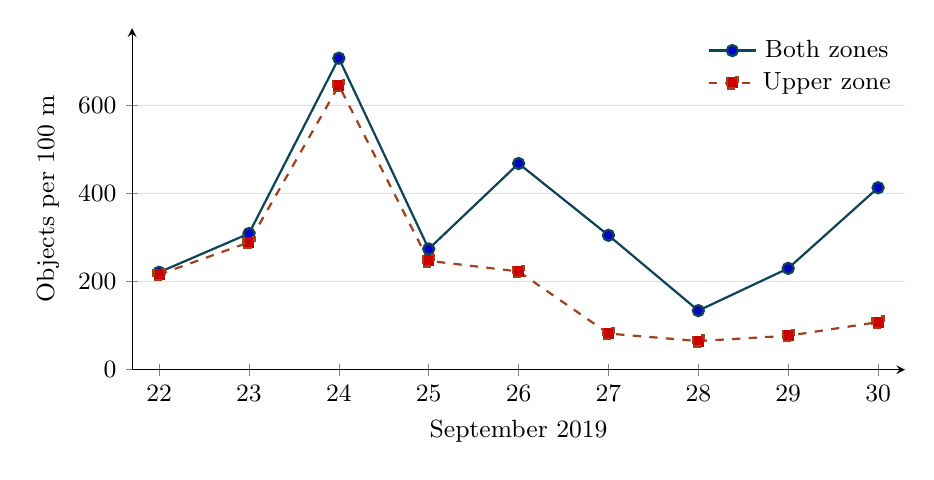
\begin{tikzpicture}
\begin{axis}[width=.94\linewidth,height=2.33in,axis lines=left,ymin=0,ymax=775,
  xlabel={September 2019},ylabel={Objects per 100 m},xmin=21.7,xmax=30.3,
  xtick={22,23,24,25,26,27,28,29,30},ytick={0,200,400,600},
  tick label style={font=\small},label style={font=\small},
  legend style={draw=none,anchor=north east,at={(1,1)},font=\small},
  ymajorgrids,grid style={gray!25}]
\addplot+[deep,thick,mark=*] coordinates {(22,221)(23,309)(24,707)(25,274)(26,468)(27,305)(28,134)(29,230)(30,413)};
\addlegendentry{Both zones}
\addplot+[warm,thick,dashed,mark=square*] coordinates {(22,216)(23,289)(24,645)(25,247)(26,223)(27,82)(28,65)(29,77)(30,108)};
\addlegendentry{Upper zone}
\end{axis}
\end{tikzpicture}\\
{\small Figure 1. Each point is one day of observed removal at uMhlanga.}
\end{center}

For a proposed fixed multiplier $c$, the relative error on visit $i$ is
$|c\,p_i-1|$ with $p_i=U_i/T_i$. Its maximum over the observations is attained at one of the two extreme shares. Equating the endpoint errors gives
\[
c^*=\frac{2}{p_{\min}+p_{\max}},\qquad
\min_{c\ge 0}\max_i |c\,p_i-1|=\frac{p_{\max}-p_{\min}}{p_{\max}+p_{\min}} .
\]
At uMhlanga the extremes are $108/413$ and $216/221$. The sharp error is $605/1047$ (57.78\%). A factor calibrated to the first four visits underestimates the combined count on the last five visits by 61.27\%. Across every chronological split retaining at least three visits on each side, the understatement there ranges from 52.70\% to 62.52\%. These comparisons apply to the catches under the original full-width clearance history.

\para{Independent seasonal evidence.}
Buoninsegni et al.\ collected items in bags by geomorphological zone on the northern Adriatic coast. Their swash zone marks wave action and differs from the South African tide-line division. We compared the published full count with the count inland of the swash. We used the four seasonal totals in Table 2 and zone areas and densities in Tables A1--A4. For a printed density $d$ and area $a$ with two decimal places, the compatible integer swash count lies between
$\lceil\max(0,d-.005)(a-.005)\rceil$ and $\lfloor(d+.005)(a+.005)\rfloor$.

Goro contained only a swash zone. Spina's summer 2024 survey omitted the dune crest. Excluding these observations left eight adjacent comparisons, including Volano's autumn survey in which the two backshore zones were combined. One showed a strict reversal throughout the rounding intervals. At Spina the full count rose from 653 in autumn 2023 to 727 in winter 2024. Swash density rose from 0.00 to 0.25 items/m$^2$ over 476.44\,m$^2$. Between zero and two autumn items and 117--121 winter items are compatible with those densities. The inland count therefore \emph{fell by 41--47} as the full count rose by 74. The printed Clean Coast Indices give a decline of 47 under the same rounding convention. For Volano, the printed winter count is 493, while the other three counts and the text's four-season total imply 439. Both values gave the same direction in the two comparisons they affect. The Spina calculation uses its own reported counts.
\src{https://www.mdpi.com/2073-4441/17/15/2173}{Buoninsegni et al., Tables 2 and A1--A4}

\newpage
\para{Counting a random subset of bags.}
A team interested in a \emph{site-period total} could still remove and label the catch in both zones at every visit. Count all upper-zone catches. At each site independently, select $k$ of $N$ dates uniformly without replacement for counting the lower-zone catches $L_i$. If all labeled bags from a chosen date remain available, the expansion estimator
\[
\widehat T=\sum_{i=1}^{N}U_i+\frac{N}{k}\sum_{i\in S}L_i
\]
is unbiased conditional on the full set of catches, because each date's inclusion probability is $k/N$. This use of inverse inclusion probabilities follows Horvitz and Thompson. We enumerated every subset of dates in the South African field records, retaining repeated subset totals with their correct multiplicity. We counted a success when \emph{both} site-period estimates were within 20\% of their observed totals. Independent selection across sites allows the two success fractions to be multiplied.
\src{https://doi.org/10.1080/01621459.1952.10483446}{Horvitz and Thompson, 1952}

\begin{center}
\begin{tabular}{rrrrl}\toprule
\multicolumn{2}{c}{Lower-zone dates counted} & \multicolumn{2}{c}{Success at each site} & Both sites\\
Amanzimtoti & uMhlanga & Amanzimtoti & uMhlanga & within 20\%\\\midrule
3 of 10 & 5 of 9 & 115/120 & 121/126 & 92.03\%\\
3 of 10 & 6 of 9 & 115/120 & 84/84 & 95.83\%\\
4 of 10 & 5 of 9 & 209/210 & 121/126 & 95.57\%\\\bottomrule
\end{tabular}
\end{center}

The first row gives the highest joint success fraction among all allocations of at most eight lower-zone counts. The other two rows are all allocations of at most nine that meet the 95\% target. At nine, the team would count 28 zone-by-date catches instead of 38, while clearing both zones at all 19 site visits. Time, storage costs and operational feasibility were not measured. Omitting counts loses daily information. Sampling cannot reconstruct each day's full trajectory. A concentration of lower-zone litter on a few other days can change the required budget.

\para{Sensitivity and inference.}
The deposited material subtotals differ from the sum of the numeric item cells in 15 of the 38 zone-by-date catches. Substituting them preserves the five daily reversals, the uMhlanga error floor and both qualifying nine-count allocations with their exact joint probabilities. One exported weight of 15,000\,kg for large wood is unresolved. The analysis uses item counts throughout. The two Italian seasons provide an independent observation of a sign reversal under a separately defined sampling boundary. The studies differ in geography, season, frequency, size thresholds and removal history. Neither establishes the rate of new marine arrivals or a causal effect of cleaning on the following visit.

\para{Verification and contributions.}
The archive includes the source snapshots and their licences, code for two independent South African reconstructions, the Italian rounding calculation, and a Lean 4 formalization of the correction bound, allocation threshold and Spina sign calculation. An independent Rust kernel rechecked the proofs. Input selection is verified separately against the published data. The field teams collected the original observations. Yoshiaki Otsuka set the research direction. Codex GPT-6.2-Sol located and analysed the South African deposit. GPT-6.2-Astra independently replayed its counts, designed the audit, analysed the Italian tables and prepared this note and formal proofs. The analyses ran locally on an Apple M3 Pro on 27 November 2026 (Japan time). Our literature check did not locate these exact calculations in earlier work. External peer review and prospective field validation are pending.
\end{document}
